\section{RRTDual  Class Reference}
\label{classRRTDual}\index{RRTDual@{RRTDual}}
Planners that grow trees from the initial and goal. 


{\tt \#include $<$rrt.h$>$}

Inheritance diagram for RRTDual::\begin{figure}[H]
\begin{center}
\leavevmode
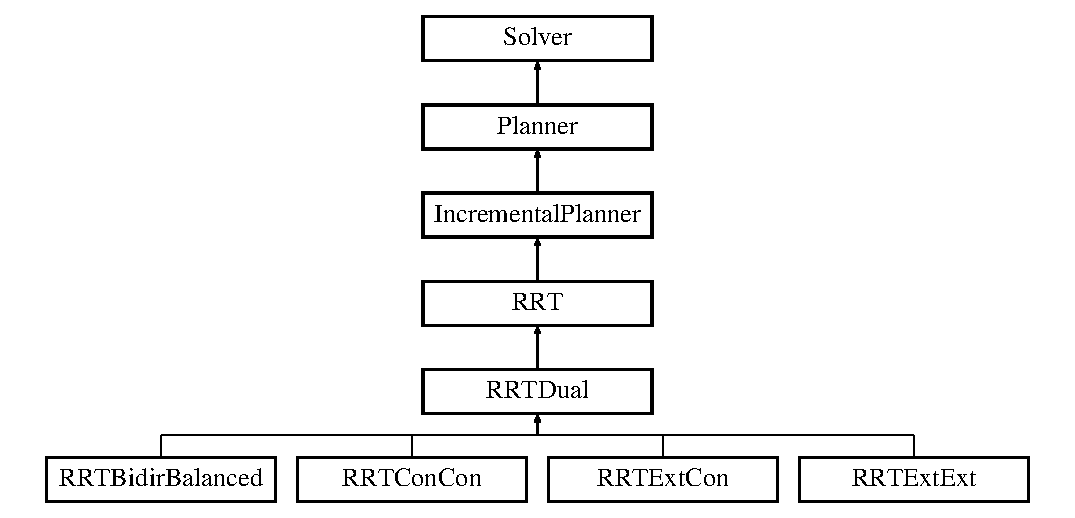
\includegraphics[height=6cm]{classRRTDual}
\end{center}
\end{figure}
\subsection*{Public Methods}
\begin{CompactItemize}
\item 
{\bf RRTDual} ({\bf Problem} $\ast$p)
\item 
virtual {\bf $\sim$RRTDual} ()
\item 
virtual bool {\bf Plan} ()
\begin{CompactList}\small\item\em The dual-tree planner used in La\-Valle, Kuffner, ICRA 1999. Each tree is extended toward a randomly-sampled point. {\bf RRTExt\-Ext} {\rm (p.\,\pageref{classRRTExtExt})} is generally better.\item\end{CompactList}\end{CompactItemize}
\subsection*{Protected Methods}
\begin{CompactItemize}
\item 
void {\bf Recover\-Solution} ({\bf MSLNode} $\ast$n1, {\bf MSLNode} $\ast$n2)
\end{CompactItemize}


\subsection{Detailed Description}
Planners that grow trees from the initial and goal.

This planner grows one tree, G, from the initial state,  and one tree, G2, from the goal state. When the closest pair of points between the two trees is within Gap\-Error, a solution path is returned. The planners in the derived classes also use two trees, and are generally more efficient than RRTDual. 



\subsection{Constructor \& Destructor Documentation}
\index{RRTDual@{RRTDual}!RRTDual@{RRTDual}}
\index{RRTDual@{RRTDual}!RRTDual@{RRTDual}}
\subsubsection{\setlength{\rightskip}{0pt plus 5cm}RRTDual::RRTDual ({\bf Problem} $\ast$ {\em p})}\label{classRRTDual_a0}


\index{RRTDual@{RRTDual}!~RRTDual@{$\sim$RRTDual}}
\index{~RRTDual@{$\sim$RRTDual}!RRTDual@{RRTDual}}
\subsubsection{\setlength{\rightskip}{0pt plus 5cm}RRTDual::$\sim$RRTDual ()\hspace{0.3cm}{\tt  [inline, virtual]}}\label{classRRTDual_a1}




\subsection{Member Function Documentation}
\index{RRTDual@{RRTDual}!Plan@{Plan}}
\index{Plan@{Plan}!RRTDual@{RRTDual}}
\subsubsection{\setlength{\rightskip}{0pt plus 5cm}bool RRTDual::Plan ()\hspace{0.3cm}{\tt  [virtual]}}\label{classRRTDual_a2}


The dual-tree planner used in La\-Valle, Kuffner, ICRA 1999. Each tree is extended toward a randomly-sampled point. {\bf RRTExt\-Ext} {\rm (p.\,\pageref{classRRTExtExt})} is generally better.



Reimplemented from {\bf RRT} {\rm (p.\,\pageref{classRRT_a3})}.

Reimplemented in {\bf RRTExt\-Ext} {\rm (p.\,\pageref{classRRTExtExt_a2})}, {\bf RRTExt\-Con} {\rm (p.\,\pageref{classRRTExtCon_a2})}, {\bf RRTCon\-Con} {\rm (p.\,\pageref{classRRTConCon_a2})}, and {\bf RRTBidir\-Balanced} {\rm (p.\,\pageref{classRRTBidirBalanced_a2})}.\index{RRTDual@{RRTDual}!RecoverSolution@{RecoverSolution}}
\index{RecoverSolution@{RecoverSolution}!RRTDual@{RRTDual}}
\subsubsection{\setlength{\rightskip}{0pt plus 5cm}void RRTDual::Recover\-Solution ({\bf MSLNode} $\ast$ {\em n1}, {\bf MSLNode} $\ast$ {\em n2})\hspace{0.3cm}{\tt  [protected]}}\label{classRRTDual_b0}




The documentation for this class was generated from the following files:\begin{CompactItemize}
\item 
{\bf rrt.h}\item 
{\bf rrt.C}\end{CompactItemize}
